I have found a code of non equilibrium DMFT IPT developed by Naoto Tsuji. This code was attached as supplementary material of their 2014 RMP paper. I have tried to reproduce the interaction quench study in paramagnetic HM, which they have published in PRL \cite{HUB_para} paper 2009.

 I have attached  figures of time evolution  double occupancy for different interaction quench.   In the public version of code they have implemented bare 2 nd order perturbation theory with Kadanoff-Baym formalism.

Their study shows that for large interaction  bare 4 th order perturbation theory give qualitative same result as QMC.

I have been thinking i can study the IHM paramagnetic case $\delta$ quenching for small U with this 2 nd order perturbation theory code.

\begin{figure}[H]
%\includegraphics[width=0.8\linewidth]{HF/gap_vs_U_HFvsIPT_t200.eps}
  \caption{}
\end{figure}

\begin{figure}[H]
%\centering
\begin{subfigure}{.5\textwidth}
 % \centering
 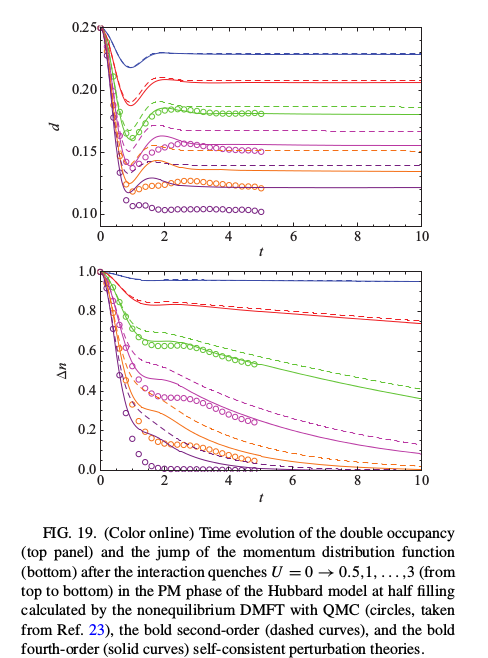
\includegraphics[width=1.1\linewidth]{bench_marking/HUB_para_quench_literature_small_U.png}
  \caption{}
  %\label{fig:sub1}
\end{subfigure}%
\begin{subfigure}{.5\textwidth}
 % \centering
  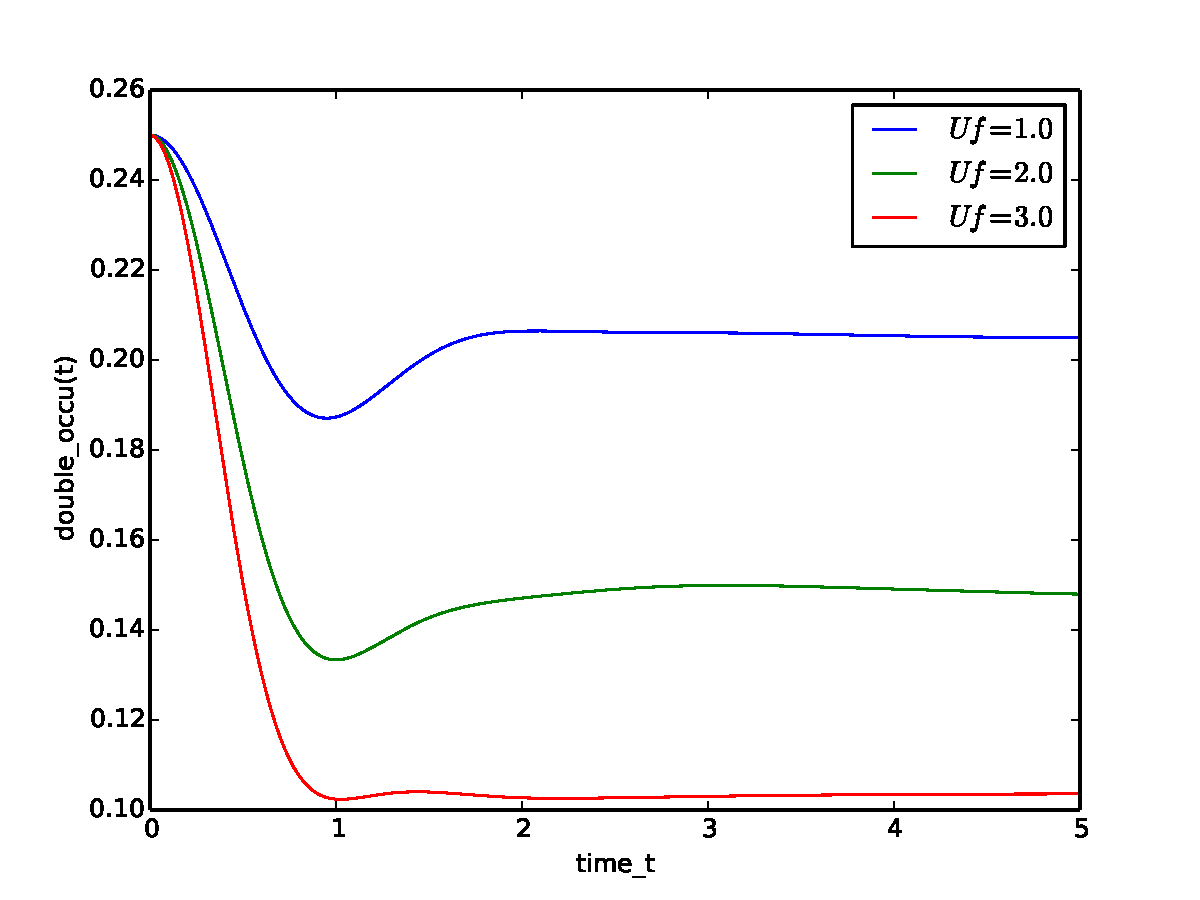
\includegraphics[width=1.1\linewidth]{bench_marking/HUB_para_quench_code_small_U.pdf}
  \caption{}
  %\label{fig:sub2}
\end{subfigure}
%\caption{dos for $\Delta=1.0t$, $t_2 = 0.4t$(a) at U = 0.4t band insulator  (b) at U = 2.0t metal}
%\label{fig:test}
\end{figure}

\begin{figure}[H]
%\includegraphics[width=0.8\linewidth]{HF/gap_vs_U_HFvsIPT_t200.eps}
  \caption{}
\end{figure}

\begin{figure}[H]
%\centering
\begin{subfigure}{.5\textwidth}
 % \centering
 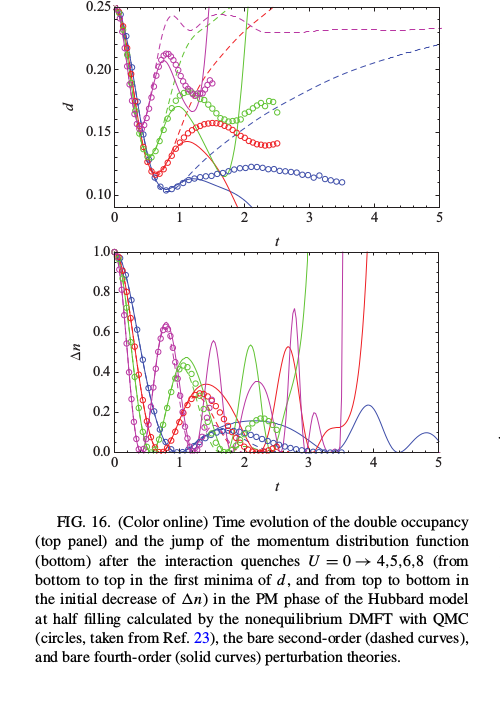
\includegraphics[width=1.1\linewidth]{bench_marking/HUB_para_quench_literature_large_U.png}
  \caption{}
  %\label{fig:sub1}
\end{subfigure}%
\begin{subfigure}{.5\textwidth}
 % \centering
  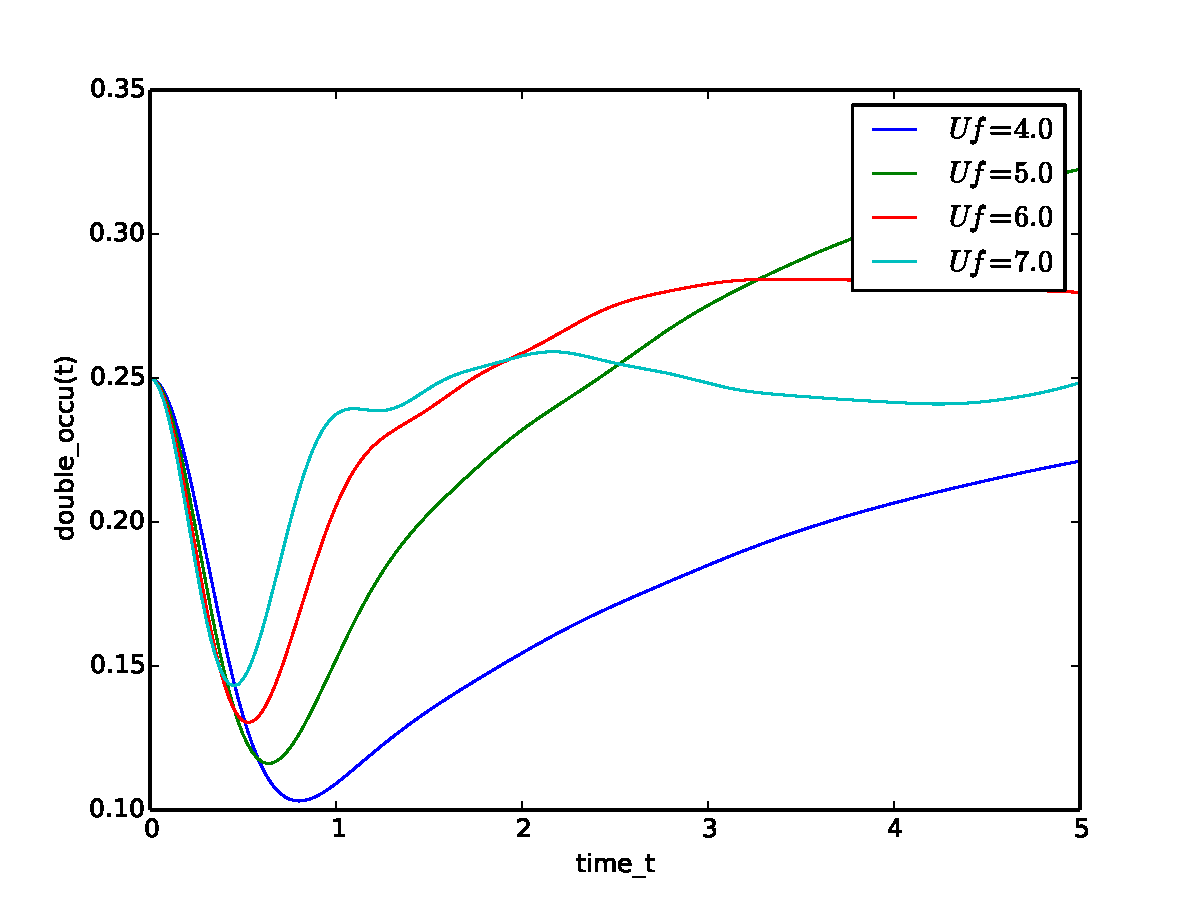
\includegraphics[width=1.1\linewidth]{bench_marking/HUB_para_quench_code_large_U.pdf}
  \caption{}
  %\label{fig:sub2}
\end{subfigure}
%\caption{dos for $\Delta=1.0t$, $t_2 = 0.4t$(a) at U = 0.4t band insulator  (b) at U = 2.0t metal}
%\label{fig:test}
\end{figure}

